\section{Survey}
\subsection*{Survey}

\begin{frame}{{\sffamily Levantamento (Survey)}}
  \begin{block}{Por que um levantamento?}
    \begin{itemize}
      \item Generalizar sobre as crenças e opiniões de muitas pessoas estudando apenas um subconjunto delas.
    \end{itemize}
  \end{block}
  \begin{block}{Objetivo}
    \begin{itemize}
      \item Entender as necessidades de alunos e professores em relação a projetos e atividades de extensão.
    \end{itemize}
  \end{block}
  Conduzido por dois alunos: Igor Costa e Lucas Fell.
\end{frame}

\begin{frame}{{\sffamily Objetivos e Estrutura}}
  \begin{block}{Objetivo de pesquisa}
    \begin{itemize}
      \item Ordenar e refinar os requisitos elicitados na revisão sistemática
    \end{itemize}
  \end{block}
  \begin{block}{Estrutura do questionário}
    \begin{itemize}
      \item Histórias de usuário
            \SubItem{Ranqueamento MoSCoW adaptado (InIDeIr)}
      \item Sugestões livres mais elaboradas
    \end{itemize}
  \end{block}
\end{frame}

\begin{frame}{{\sffamily Identificação e Questões}}
  \begin{block}{Identificação}
    \begin{itemize}
      \item Público alvo
            \SubItem{Comunidade acadêmica}
      \item Dados de identificação
            \SubItem{Gênero, educação, faixa etária, papel na extensão}
      \item Separação da amostra
            \SubItem{Discentes, Docentes e TAEs}
    \end{itemize}
  \end{block}
\end{frame}

\begin{frame}{{\sffamily Identificação e Questões}}
  \begin{block}{Questões}
    \begin{itemize}
      \item Discentes: 14 questões
      \item Docentes/TAEs: 11 questões
    \end{itemize}
  \end{block}
\end{frame}


\begin{frame}{{\sffamily Identificação e Questões}}

\begin{columns}
\begin{column}{0.5\textwidth}
   \begin{figure}
        \centering
        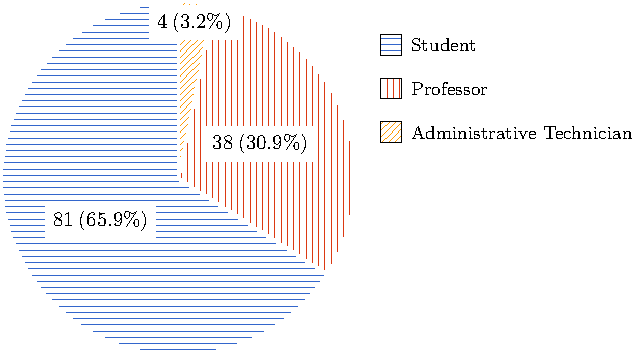
\includegraphics[width=6cm, ]{imagens/5-community-roles.pdf}
    \end{figure}
\end{column}
\begin{column}{0.5\textwidth}  %%<--- here
\begin{figure}
        \centering
        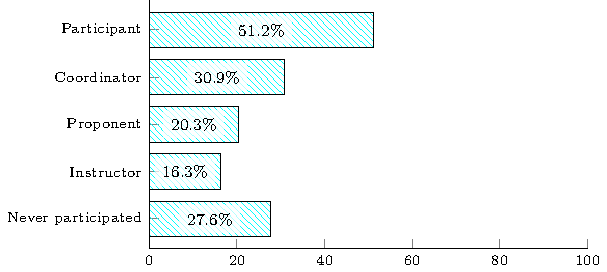
\includegraphics[width=5.5cm, ]{imagens/5-outreach-roles.pdf}
    \end{figure}
    % \begin{center}
    %  \includegraphics[width=0.5\textwidth]{image1.jpg}
    %  \end{center}
\end{column}
\end{columns}
\end{frame}


% \begin{frame}{{\sffamily Identificação e Questões}}
%   \
% \end{frame}

\begin{frame}{{\sffamily Resultados}}
  \begin{block}{Resultados}
    \begin{itemize}
      \item 123 respostas no total
      \item 23\% e 12\% de respostas qualitativas para professores e alunos, respectivamente
    \end{itemize}
  \end{block}
\end{frame}

\begin{frame}{{\sffamily Resultados - Análise quantitativa}}
  \begin{block}{Questão 1 dos docentes/TAEs}
    ``P1 - Eu como Proponente, gostaria de propor uma atividade de extensão, criando oportunidades de conhecimento para outras pessoas.''
  \end{block}
\end{frame}

\begin{frame}{{\sffamily Resultados - Análise quantitativa}}
  \begin{figure}
    \centering
    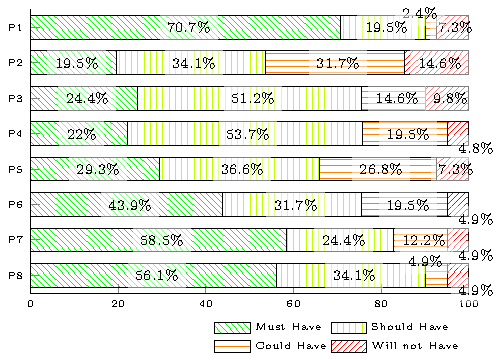
\includegraphics[width=8cm, ]{imagens/5-questions-proponent.pdf}
  \end{figure}
\end{frame}

\begin{frame}{{\sffamily Resultados - Análise quantitativa}}
  \begin{block}{Questão 11 dos alunos}
    ``A11 - Eu como Participante, gostaria de realizar a inscrição em atividades de extensão sem fazer cadastro no sistema, para que minhas informações não sejam salvas.''
  \end{block}
\end{frame}

\begin{frame}{{\sffamily Resultados - Análise quantitativa}}
  \begin{figure}
    \centering
    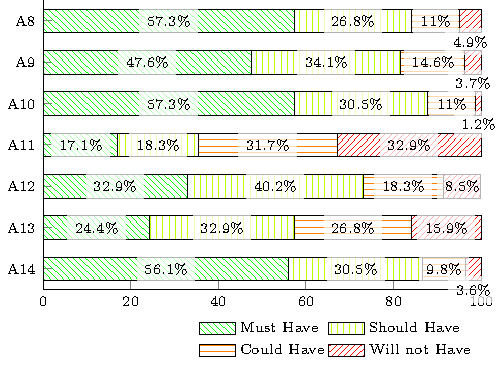
\includegraphics[width=8cm, ]{imagens/5-questions-participant-2.pdf}
  \end{figure}
\end{frame}

\begin{frame}{{\sffamily Resultados - Análise qualitativa}}
  Novos requisitos levantados baseado nas sugestões:
  \begin{block}{Professores/TAEs}
    \begin{itemize}
      \item Geração de certificados em conjunto
      \item Geração de relatórios no formato do programa SAP
      \item Priorização de participantes
      \item Certificado de inscrição
    \end{itemize}
  \end{block}
  \begin{block}{Alunos}
    \begin{itemize}
      \item Notificações (prazo de inscrição)
    \end{itemize}
  \end{block}
\end{frame}

\begin{frame}{{\sffamily Ameaças à validade}}
  \begin{block}{Ameaças à validade}
    \begin{itemize}
      \item Escala MoSCoW
            \SubItem{Engenharia de Software}
      \item Histórias de usuário muito descritas
            \SubItem{Difícil de encontrar novas funcionalidades}
      \item Falta de clareza nos termos
    \end{itemize}
  \end{block}
\end{frame}